\documentclass[11pt,a4paper]{article}

\usepackage[T1]{fontenc}
\usepackage{lmodern}
\usepackage[margin=2.5cm]{geometry}
\usepackage{amsmath,amssymb,amsthm,mathtools,bm}
\usepackage{booktabs}
\usepackage{graphicx}
\usepackage{xcolor}
\usepackage{microtype}
\usepackage{enumitem}
\usepackage[font=small,labelfont=bf]{caption}
\usepackage{algorithm}
\usepackage{algpseudocode}
\usepackage[numbers,sort&compress]{natbib}
\usepackage[colorlinks=true,linkcolor=blue!50!black,citecolor=blue!50!black,urlcolor=blue!50!black]{hyperref}
\usepackage[capitalise,noabbrev]{cleveref}
\algdef{SE}[PARFOR]{ParFor}{EndParFor}[1]{\textbf{parallel for} #1 \textbf{do}}{\textbf{end parallel for}}

\hypersetup{pdftitle={Monte Carlo Pricing of European Options},pdfauthor={Kevin Feltrin},
  pdfsubject={Convergence, variance reduction and Greeks against the Black-Scholes benchmark},
  pdfkeywords={Monte Carlo, Black-Scholes, variance reduction, Greeks, quasi-Monte Carlo}}

% Generated by scripts/make_figures.py -- do not edit by hand.
\newcommand{\BSPrice}{10.4506}
\newcommand{\TablePaths}{2^{22}}
\newcommand{\VRFAnti}{2.00}
\newcommand{\EffAnti}{3.69}
\newcommand{\VRFCV}{6.89}
\newcommand{\EffCV}{6.30}
\newcommand{\VRFBoth}{28.7}
\newcommand{\EffBoth}{53.5}
\newcommand{\RhoCV}{0.925}
\newcommand{\BetaCV}{0.674}
\newcommand{\TheoryVRFCV}{6.89}
\newcommand{\CrudeSE}{0.0072}
\newcommand{\BothSE}{0.00134}
\newcommand{\VRFAntiCallLow}{17.2}
\newcommand{\VRFAntiCallHigh}{1.07}
\newcommand{\VRFCVCallLow}{420}
\newcommand{\VRFCVCallHigh}{1.69}
\newcommand{\VRFBothCallLow}{938}
\newcommand{\VRFBothCallHigh}{13.4}
\newcommand{\VRFAntiPutLow}{1.01}
\newcommand{\VRFAntiPutHigh}{49.9}
\newcommand{\VRFCVPutLow}{1.07}
\newcommand{\VRFCVPutHigh}{12.7}
\newcommand{\VRFBothPutLow}{2.39}
\newcommand{\VRFBothPutHigh}{101}
\newcommand{\DeltaCRNVarianceGain}{332}
\newcommand{\GammaCRNVarianceGain}{112\,521}
\newcommand{\DeltaLRVarianceRatio}{6.5}
\newcommand{\AsianVRFAnti}{2.08}
\newcommand{\AsianVRFCV}{1\,301}
\newcommand{\AsianVRFBoth}{1\,197}
\newcommand{\AsianEffCV}{1\,247}
\newcommand{\AsianRhoCV}{0.9996}
\newcommand{\AsianRhoBoth}{0.9991}
\newcommand{\AsianBetaCV}{1.031}
\newcommand{\AsianGeoPrice}{5.9402}
\newcommand{\AsianRefPrice}{$6.156058 \pm 0.000043$}
\newcommand{\PerfPaths}{2^{24}}
\newcommand{\ThroughputSerial}{9.3}
\newcommand{\ThroughputParallel}{125}
\newcommand{\SpeedupMax}{13.5}
\newcommand{\ThreadsBest}{16}
\newcommand{\ThreadsMax}{16}
\newcommand{\AllIdentical}{yes}
\newcommand{\CompilerName}{MSVC 19.43}
\newcommand{\CPUName}{12th Gen Intel Core i7-1260P}
\newcommand{\SlopeCrude}{\ensuremath{-0.496}}
\newcommand{\SlopeAntithetic}{\ensuremath{-0.499}}
\newcommand{\SlopeControlVariate}{\ensuremath{-0.497}}
\newcommand{\SlopeAntitheticControlVariate}{\ensuremath{-0.503}}
\newcommand{\CoverageMin}{0.926}
\newcommand{\CoverageMax}{0.964}
\newcommand{\CoverageSmallCrude}{0.940}
\newcommand{\Replications}{500}
\newcommand{\MaxConvergencePaths}{2^{20}}
\newcommand{\MinConvergencePaths}{2^{7}}
\newcommand{\SeOverRmseMin}{0.96}
\newcommand{\SeOverRmseMax}{1.04}
\newcommand{\BestDeltaH}{0.013}
\newcommand{\BestDeltaRmse}{0.0023}
\newcommand{\BestDeltaIndepRmse}{0.0073}
\newcommand{\BestDeltaIndepH}{0.063}
\newcommand{\DeltaPathwiseRmse}{0.0023}
\newcommand{\DeltaLikelihoodRatioRmse}{0.0061}
\newcommand{\BestGammaH}{0.063}
\newcommand{\BestGammaRmse}{0.00019}
\newcommand{\BestGammaIndepRmse}{0.00082}
\newcommand{\BestGammaIndepH}{0.14}
\newcommand{\GammaLikelihoodRatioRmse}{0.00059}
\newcommand{\GreekBumpPaths}{2^{16}}
\newcommand{\GreekReplications}{200}
\newcommand{\SlopeRQMC}{\ensuremath{-0.934}}
\newcommand{\RQMCGainAtMax}{271}
\newcommand{\RQMCVarianceGainAtMax}{73\,493}


% ------------------------------------------------------------------ notation
\newcommand{\E}{\mathbb{E}}
\newcommand{\Var}{\operatorname{Var}}
\newcommand{\Cov}{\operatorname{Cov}}
\newcommand{\Corr}{\operatorname{Corr}}
\newcommand{\Q}{\mathbb{Q}}
\newcommand{\N}{\mathcal{N}}
\newcommand{\1}{\mathbf{1}}
\newcommand{\dd}{\,\mathrm{d}}
\newcommand{\repo}{\url{https://github.com/KvnFltr/monte-carlo-option-pricer}}

\theoremstyle{plain}
\newtheorem{proposition}{Proposition}
\theoremstyle{remark}
\newtheorem*{remark}{Remark}

\title{\textbf{Monte Carlo Pricing of European Options}\\[4pt]
  \large Convergence, Variance Reduction and Greeks\\ against the Black--Scholes Benchmark}
\author{Kevin Feltrin}
\date{November 2026}

\begin{document}
\maketitle

\begin{abstract}
\noindent
We implement in C++20 a Monte Carlo pricer for European options in the Black--Scholes model and use the
closed-form price as ground truth to measure the statistical behaviour of the estimators. Over
\Replications{} independent replications per sample size, the root-mean-square error of the crude
estimator decays as $N^{\SlopeCrude}$, in agreement with the $\mathcal{O}(N^{-1/2})$ rate of the central limit
theorem, and the asymptotic 95\% confidence intervals have an empirical coverage between \CoverageMin{} and
\CoverageMax{} for $N \ge 2^{14}$. For an at-the-money call, antithetic variates, a control variate on the
terminal price and their combination reduce the variance by factors of \VRFAnti, \VRFCV{} and \VRFBoth;
once the cost of each method is accounted for, the efficiency gain reaches \EffBoth. Greeks are computed by
central finite differences: common random numbers divide the variance of the Delta estimator by
\DeltaCRNVarianceGain{} and that of Gamma by about five orders of magnitude, and we characterise the
bias--variance trade-off in the bump size against pathwise and likelihood-ratio estimators. Two extensions show
where these tools matter in practice: an arithmetic Asian option, for which the geometric control variate
reduces the variance by a factor of \AsianVRFCV, and a randomised quasi-Monte Carlo estimator whose error
decays as $N^{\SlopeRQMC}$. Random numbers come from the counter-based generator Philox4x32-10, which makes
every result bitwise reproducible whatever the number of threads. Code, tests and the scripts producing every
figure and table of this report are available at \repo.
\end{abstract}

\tableofcontents
\bigskip

% =====================================================================================================
\section{Introduction}

Monte Carlo simulation, introduced in option pricing by \citet{boyle1977}, is the method of choice when the
payoff depends on the whole path of the underlying or on many risk factors: its convergence rate
$\mathcal{O}(N^{-1/2})$ does not depend on the dimension, unlike lattice or PDE methods. The price to pay is a
slow and noisy convergence, so the practical value of a Monte Carlo engine lies in three things: an honest
error estimate, variance reduction, and stable sensitivities.

A European option in the Black--Scholes model \citep{black1973,merton1973} is the ideal laboratory to study
them, because its price and Greeks are known in closed form. The exact error of every estimator can therefore
be measured, not just estimated. This report uses that benchmark to answer four questions:
\begin{enumerate}[nosep]
  \item Does the error decay as $N^{-1/2}$, and are the confidence intervals reliable (\cref{sec:convergence})?
  \item How much do antithetic variates and control variates reduce the variance, and at what cost
        (\cref{sec:vr,sec:res-vr})?
  \item How should the bump of a finite-difference Greek be chosen, and what do common random numbers bring
        (\cref{sec:greeks,sec:res-greeks})?
  \item What changes for a path-dependent payoff and for quasi-random points (\cref{sec:res-asian,sec:res-qmc})?
\end{enumerate}
\Cref{sec:implementation} describes the implementation, in particular the use of a counter-based random number
generator to obtain parallel simulations that are reproducible to the last bit.

% =====================================================================================================
\section{The Black--Scholes benchmark}\label{sec:bs}

Under the risk-neutral measure $\Q$, the underlying follows a geometric Brownian motion with continuous
dividend yield $q$,
\begin{equation}
  \dd S_t = (r - q)\, S_t \dd t + \sigma S_t \dd W_t,
  \qquad
  S_T = S_0 \exp\!\Big( \big(r - q - \tfrac{1}{2}\sigma^2\big) T + \sigma \sqrt{T}\, Z \Big),
  \quad Z \sim \N(0,1).
  \label{eq:gbm}
\end{equation}
The price of a claim paying $f(S_T)$ at $T$ is $V = \E^{\Q}[e^{-rT} f(S_T)]$. For the call
$f(s) = (s-K)^+$ and the put $f(s) = (K-s)^+$,
\begin{equation}
  C = S_0 e^{-qT} \Phi(d_1) - K e^{-rT} \Phi(d_2), \qquad
  P = K e^{-rT} \Phi(-d_2) - S_0 e^{-qT} \Phi(-d_1),
  \label{eq:bs}
\end{equation}
with $d_{1,2} = \big[\ln(S_0/K) + (r - q \pm \sigma^2/2) T\big] / (\sigma\sqrt{T})$ and $\Phi$ the standard
normal distribution function. The sensitivities used as reference are listed in \cref{tab:greeks-formulas}.

\begin{table}[ht]
\centering
\caption{Closed-form Greeks of European options ($\varphi$ is the standard normal density). Vega and rho are
per unit change; theta is the derivative with respect to calendar time, $\Theta = -\partial V/\partial T$, and
$\Theta_0 = -S_0 e^{-qT}\varphi(d_1)\,\sigma/(2\sqrt{T})$.}
\label{tab:greeks-formulas}
\small
\renewcommand{\arraystretch}{1.25}
\begin{tabular}{lll}
\toprule
Greek & Call & Put \\
\midrule
$\Delta = \partial V/\partial S_0$ & $e^{-qT}\Phi(d_1)$ & $-e^{-qT}\Phi(-d_1)$ \\
$\Gamma = \partial^2 V/\partial S_0^2$ & \multicolumn{2}{c}{$e^{-qT}\varphi(d_1) / (S_0 \sigma \sqrt{T})$} \\
$\mathcal{V} = \partial V/\partial \sigma$ & \multicolumn{2}{c}{$S_0 e^{-qT} \varphi(d_1)\sqrt{T}$} \\
$\rho = \partial V/\partial r$ & $K T e^{-rT}\Phi(d_2)$ & $-K T e^{-rT}\Phi(-d_2)$ \\
$\Theta = -\partial V/\partial T$ & $\Theta_0 - rKe^{-rT}\Phi(d_2) + qS_0e^{-qT}\Phi(d_1)$
         & $\Theta_0 + rKe^{-rT}\Phi(-d_2) - qS_0e^{-qT}\Phi(-d_1)$ \\
\bottomrule
\end{tabular}
\end{table}

Unless stated otherwise, the experiments use $S_0 = K = 100$, $r = 5\%$, $q = 0$, $\sigma = 20\%$ and $T = 1$,
for which the call is worth $C = \BSPrice$.

% =====================================================================================================
\section{Monte Carlo estimation}\label{sec:mc}

\subsection{Estimator and confidence interval}

Let $Y = e^{-rT} f(S_T)$ be the discounted payoff. Since $S_T$ in \eqref{eq:gbm} is an explicit function of a
single Gaussian variable, it can be sampled exactly: there is no time-discretisation bias and the only error is
statistical. With $N$ independent copies $Y_1, \dots, Y_N$, the crude estimator
\begin{equation}
  \hat V_N = \frac{1}{N} \sum_{i=1}^N Y_i
\end{equation}
is unbiased, converges almost surely by the strong law of large numbers and, since $\sigma_Y^2 = \Var(Y) <
\infty$, satisfies the central limit theorem
\begin{equation}
  \sqrt{N}\,\big(\hat V_N - V\big) \xrightarrow{\;d\;} \N(0, \sigma_Y^2).
\end{equation}
Its root-mean-square error is exactly $\sigma_Y/\sqrt{N}$: one more correct digit costs a hundred times more
paths. Replacing $\sigma_Y$ by the sample standard deviation $s_N$ gives the asymptotic confidence interval
$\hat V_N \pm z_{0.975}\, s_N/\sqrt{N}$ with $z_{0.975} \approx 1.96$. Its coverage is only asymptotically
95\%: for small $N$ the skewness of the payoff distorts it, which \cref{sec:convergence} quantifies.

\subsection{Efficiency}

A variance reduction technique is worth using only if it lowers the variance more than it raises the cost.
Following \citet{glynn1992}, the efficiency of an estimator is the inverse of its work-normalised variance
$\sigma^2 \tau$, where $\sigma^2$ is the variance per path and $\tau$ the computing time per path. We report the
\emph{variance reduction factor} (VRF), $\sigma^2_{\text{crude}}/\sigma^2$ at an equal number of payoff
evaluations, and the \emph{efficiency gain}
\begin{equation}
  \text{Efficiency} = \frac{\sigma^2_{\text{crude}}\, \tau_{\text{crude}}}{\sigma^2\, \tau},
  \label{eq:efficiency}
\end{equation}
which is the factor by which the computing time needed for a given accuracy is divided.

% =====================================================================================================
\section{Variance reduction}\label{sec:vr}

\subsection{Antithetic variates}

Since $Z$ and $-Z$ have the same distribution, each draw can be used twice \citep{hammersley1956}. With
$n = N/2$ pairs, the antithetic estimator averages $\bar Y_i = \frac12\big[f(Z_i) + f(-Z_i)\big]$, where we write
$f(Z)$ for the discounted payoff as a function of the Gaussian draw. With $\rho_A = \Corr\big(f(Z), f(-Z)\big)$,
\begin{equation}
  \Var\big(\hat V^{\text{AV}}\big) = \frac{1}{n}\cdot\frac{\sigma_Y^2 (1 + \rho_A)}{2} = \frac{\sigma_Y^2 (1+\rho_A)}{N},
  \qquad \text{VRF} = \frac{1}{1 + \rho_A}.
\end{equation}
The method helps if and only if $\rho_A < 0$, which is guaranteed for monotone payoffs.

\begin{proposition}\label{prop:antithetic}
If $f$ is monotone, then $\Cov\big(f(Z), f(-Z)\big) \le 0$; antithetic sampling never increases the variance.
\end{proposition}
\begin{proof}
Assume $f$ non-decreasing and let $Z'$ be an independent copy of $Z$. Since $z \mapsto f(-z)$ is non-increasing,
$\big(f(z) - f(z')\big)\big(f(-z) - f(-z')\big) \le 0$ for all $z, z'$. Taking expectations, the left-hand side
equals $2\Cov\big(f(Z), f(-Z)\big)$.
\end{proof}

The gain depends on how close to linear $f$ is. Deep in the money the call payoff is almost linear in $S_T$,
and for $f(Z) = a + b\,S_T$ a direct computation with the lognormal moments gives $\rho_A = -e^{-\sigma^2 T}$:
the VRF of a deep in-the-money call therefore tends to $1/(1 - e^{-\sigma^2 T}) \approx 25.5$ for our parameters.
Out of the money most pairs have both payoffs equal to zero and $\rho_A \to 0$. Antithetic sampling is also cheaper per payoff, since it needs $N/2$ Gaussian draws
instead of $N$, so its efficiency gain exceeds its VRF.

\subsection{Control variates}

Let $X$ be a variable correlated with $Y$ whose mean is known. For any $\beta$,
$\hat V^{\text{CV}}(\beta) = \bar Y - \beta (\bar X - \E X)$ is unbiased, and its variance
$\big(\sigma_Y^2 - 2\beta\Cov(Y,X) + \beta^2\sigma_X^2\big)/N$ is minimal for
\begin{equation}
  \beta^\star = \frac{\Cov(Y,X)}{\Var(X)}, \qquad
  \Var\big(\hat V^{\text{CV}}(\beta^\star)\big) = \frac{\sigma_Y^2\,(1 - \rho_{XY}^2)}{N}, \qquad
  \text{VRF} = \frac{1}{1-\rho_{XY}^2}.
  \label{eq:cv}
\end{equation}
We use the discounted terminal price $X = e^{-rT} S_T$, whose expectation $S_0 e^{-qT}$ is known because the
discounted forward is a martingale. $\beta^\star$ is estimated by least squares on the same sample, which
introduces a bias of order $1/N$ \citep[\S 4.1]{glasserman2003}, negligible next to the $N^{-1/2}$ statistical
error; the residual variance is computed with $N-2$ degrees of freedom. The estimator has a natural financial
reading: $Y - \beta X$ is the discounted value of the option hedged statically with $\beta$ units of the
underlying, so the control variate removes the part of the payoff that a delta hedge would remove, with the
regression slope in place of the Black--Scholes delta.

\subsection{Combining both}

The two techniques compose: the control variate is applied to the pair averages
$\big(\bar Y_i, \bar X_i\big)$. Antithetic averaging cancels the odd part of $f$ in $Z$, which is precisely the
part best explained by a linear control, so the two gains do not simply multiply. The combined estimator has to
be assessed empirically (\cref{sec:res-vr,sec:res-asian}).

% =====================================================================================================
\section{Greeks by simulation}\label{sec:greeks}

\subsection{Finite differences and common random numbers}

The central differences
\begin{equation}
  \hat\Delta_h = \frac{\hat V(S_0 + h) - \hat V(S_0 - h)}{2h}, \qquad
  \hat\Gamma_h = \frac{\hat V(S_0 + h) - 2\hat V(S_0) + \hat V(S_0 - h)}{h^2}
\end{equation}
have biases $\frac{h^2}{6}\,\partial_S^3 V$ and $\frac{h^2}{12}\,\partial_S^4 V$ up to $\mathcal{O}(h^4)$.
Vega, rho and theta are obtained in the same way by bumping $\sigma$, $r$ and $T$. Their variance depends
critically on how the revaluations are simulated.

\paragraph{Independent draws.}
If each $\hat V$ uses its own random numbers, $\Var(\hat\Delta_h) \approx \sigma_Y^2/(2Nh^2)$ and
$\Var(\hat\Gamma_h) \approx 6\sigma_Y^2/(Nh^4)$: the variance explodes as $h \to 0$. Balancing it with the squared
bias gives the optimal bumps $h^\star \propto N^{-1/6}$ for Delta and $N^{-1/8}$ for Gamma, and errors of order
$N^{-1/3}$ and $N^{-1/4}$ only.

\paragraph{Common random numbers (CRN).}
If the three revaluations reuse the same $Z_i$, the estimator becomes an average of per-path differences. For a
Lipschitz payoff, $|Y(S_0+h) - Y(S_0-h)| \le 2h\, e^{-rT} S_T/S_0$, so $\Var(\hat\Delta_h) = \mathcal{O}(1/N)$
uniformly in $h$: the bump can be taken small and the $N^{-1/2}$ rate is recovered \citep[\S 7.1]{glasserman2003}.
For Gamma, the per-path second difference of a call is non-zero only when $K$ lies between the bumped terminal
prices, an event of probability $\mathcal{O}(h)$, on which it is of size $\mathcal{O}(1/h)$. Hence
$\Var(\hat\Gamma_h) = \mathcal{O}\big(1/(Nh)\big)$, the optimal bump is $h^\star \propto N^{-1/5}$ and the error
decays as $N^{-2/5}$.

\subsection{Pathwise and likelihood-ratio estimators}

Two unbiased alternatives avoid the bump altogether \citep{broadie1996}.

\paragraph{Pathwise.} When the discounted payoff is almost surely differentiable in the parameter and Lipschitz,
derivative and expectation commute. For the call, with $\partial S_T/\partial S_0 = S_T/S_0$ and
$\partial S_T/\partial\sigma = S_T(\sqrt{T}Z - \sigma T)$,
\begin{equation}
  \Delta = \E\Big[e^{-rT}\1_{\{S_T > K\}} \frac{S_T}{S_0}\Big], \qquad
  \mathcal{V} = \E\Big[e^{-rT}\1_{\{S_T > K\}}\, S_T\big(\sqrt{T}Z - \sigma T\big)\Big].
\end{equation}
Rho and theta follow in the same way. The method fails for Gamma, because the derivative of the indicator is a
Dirac mass. The CRN finite-difference estimator of Delta converges path by path to the pathwise estimator as
$h \to 0$.

\paragraph{Likelihood ratio.} Differentiating the density $g_\theta$ of $S_T$ instead of the payoff gives
$\partial_\theta V = \E\big[e^{-rT} f(S_T)\, \partial_\theta \ln g_\theta(S_T)\big]$. The score weights are
\begin{equation}
  \Delta: \frac{Z}{S_0\sigma\sqrt{T}}, \qquad
  \Gamma: \frac{Z^2 - 1 - Z\sigma\sqrt{T}}{S_0^2\sigma^2 T}, \qquad
  \mathcal{V}: \frac{Z^2-1}{\sigma} - Z\sqrt{T}, \qquad
  \rho: \frac{Z\sqrt{T}}{\sigma} - T.
\end{equation}
The payoff need not be smooth, but the weights grow with $|Z|$ and so does the variance.

% =====================================================================================================
\section{Implementation}\label{sec:implementation}

The library \texttt{mcpricer} (C++20, CMake, no runtime dependency) is organised in small modules: closed forms
(\texttt{black\_scholes}), random numbers (\texttt{rng}, \texttt{normal}), streaming statistics
(\texttt{statistics}), the deterministic parallel driver (\texttt{parallel}), and the estimators
(\texttt{european}, \texttt{greeks}, \texttt{asian}, \texttt{qmc}). A command-line pricer and the driver
\texttt{run\_experiments}, which writes every result of \cref{sec:results} as CSV, are built on top of it; a
Python script turns the CSV files into the figures and tables of this report.

\subsection{Counter-based random numbers}

Random numbers come from Philox4x32-10 \citep{salmon2011}, a keyed bijection on 128-bit counters that passes the
BigCrush battery. Instead of a sequential state, the $k$-th block of random bits of path $i$ is obtained in
$\mathcal{O}(1)$ as $\mathrm{Philox}_{\text{key}=\text{seed}}(k, s, i)$, where $s$ labels a sub-stream. This
design has four consequences that the rest of the code relies on.
\begin{enumerate}[nosep]
  \item Path $i$ sees the same Gaussian draws whichever thread simulates it, so the results do not depend on the
        number of threads or on the scheduling.
  \item The simulation with $N$ paths is the prefix of every longer simulation with the same seed, which gives
        the nested estimates of \cref{fig:running} for free.
  \item Common random numbers for finite differences come by construction: the bumped and unbumped scenarios of
        path $i$ simply read the same stream. Independent scenarios read different sub-streams $s$.
  \item Each replication of an experiment uses its own seed, with no risk of overlapping sequences.
\end{enumerate}
The implementation is validated against the known-answer vectors of the reference implementation.
Uniforms are built from the top 53 bits as $(k + \frac12)\, 2^{-53}$, so they lie strictly inside $(0,1)$, and
mapped to Gaussians by inversion with Wichura's algorithm AS\,241 \citep{wichura1988}, accurate to about
$10^{-16}$. Inversion uses one uniform per Gaussian and is monotone, which keeps a one-to-one link between a
point of $(0,1)$ and a path; this is what allows quasi-random points to be used unchanged (\cref{sec:res-qmc}).

\subsection{Deterministic parallel reduction}

The paths are cut into blocks of 4096. Each block is reduced into its own accumulator, in parallel with OpenMP,
using Welford's one-pass update of the mean and of the centred second moments \citep{welford1962}, which avoids
the cancellation of the textbook formula $\sum y^2 - N\bar y^2$. The partial results are then merged
sequentially in block order with the pairwise formulas of \citet{chan1983}. Because neither the partition nor
the merge order depends on the threads, the estimate is bitwise identical for any thread count; the unit tests
check this equality, not mere closeness. Control variates use the bivariate version of the same accumulator
(means, variances and covariance).

\begin{algorithm}[ht]
\caption{Deterministic parallel Monte Carlo estimator}\label{alg:mc}
\begin{algorithmic}[1]
\Require number of paths $N$, seed, block size $B$, path function $i \mapsto Y_i$
\State $M \gets \lceil N/B \rceil$
\ParFor{$b = 0, \dots, M-1$} \Comment{OpenMP, dynamic schedule}
  \State $A_b \gets$ empty Welford accumulator
  \For{$i = bB, \dots, \min(N, (b+1)B) - 1$}
    \State $u \gets \mathrm{Philox}_{\text{seed}}(0, 0, i)$; \; $Z \gets \Phi^{-1}(u)$; \; $A_b.\mathrm{add}\big(Y(Z)\big)$
  \EndFor
\EndParFor
\State $A \gets A_0$; \textbf{for} $b = 1, \dots, M-1$: $A \gets \mathrm{merge}(A, A_b)$ \Comment{fixed order}
\State \Return $\bar Y = A.\mathrm{mean}$, \; $\mathrm{SE} = \sqrt{A.\mathrm{variance}/N}$
\end{algorithmic}
\end{algorithm}

\subsection{Testing}

The library is covered by 119 GoogleTest cases, run in continuous integration on Linux (GCC), macOS (Clang)
and Windows (MSVC), and under AddressSanitizer and UndefinedBehaviorSanitizer. They include the Philox
known-answer vectors; reference prices from \citet{hull2018} and from an independent SciPy implementation;
put--call parity; agreement of each closed-form Greek with a finite difference of the closed-form price; the
accuracy of $\Phi^{-1}$ across ten orders of magnitude; statistical tests of every estimator against the closed
form at four standard errors; the $1/\sqrt{N}$ scaling of the standard error; the empirical coverage of the
confidence interval; and bitwise reproducibility across thread counts. Because every simulation is a
deterministic function of its seed, the statistical tests are reproducible and never flaky.

% =====================================================================================================
\section{Numerical results}\label{sec:results}

All results were produced by \texttt{run\_experiments} (compiled with \CompilerName{}, \texttt{-O2}, OpenMP)
on a laptop with an \CPUName{} (\ThreadsMax{} hardware threads).

\subsection{Convergence and reliability of the error estimate}\label{sec:convergence}

For each $N = 2^7, \dots, 2^{20}$ and each method, \Replications{} independent replications (distinct seeds)
are compared with the exact price. \Cref{fig:convergence}(a) shows that the empirical RMSE decays as
$N^{-1/2}$ for all four estimators: the fitted log--log slopes over $N \ge 2^{10}$ are \SlopeCrude{} (crude),
\SlopeAntithetic{} (antithetic), \SlopeControlVariate{} (control variate) and \SlopeAntitheticControlVariate{}
(combined). Variance reduction shifts the lines down without changing their slope, as expected from
$\text{RMSE} = \sigma/\sqrt{N}$. The dashed lines, the average standard error estimated by each run, are almost
indistinguishable from the measured RMSE: their ratio lies between \SeOverRmseMin{} and \SeOverRmseMax{} for
$N \ge 2^{10}$, so the error bars reported by the pricer can be trusted.

\Cref{fig:convergence}(b) checks the 95\% confidence intervals. For $N \ge 2^{14}$ the empirical coverage lies
between \CoverageMin{} and \CoverageMax, within the binomial fluctuation range expected from \Replications{}
replications. At small sample sizes the asymptotic interval is too optimistic: with $2^7$ paths the combined
estimator covers the true price in only about 90\% of the runs, because the regression coefficient is
estimated from 64 pairs and the payoff distribution is strongly skewed. \Cref{fig:running} shows a single run
of increasing size; thanks to the counter-based generator, each point is the exact prefix of the next.

\begin{figure}[ht]
  \centering
  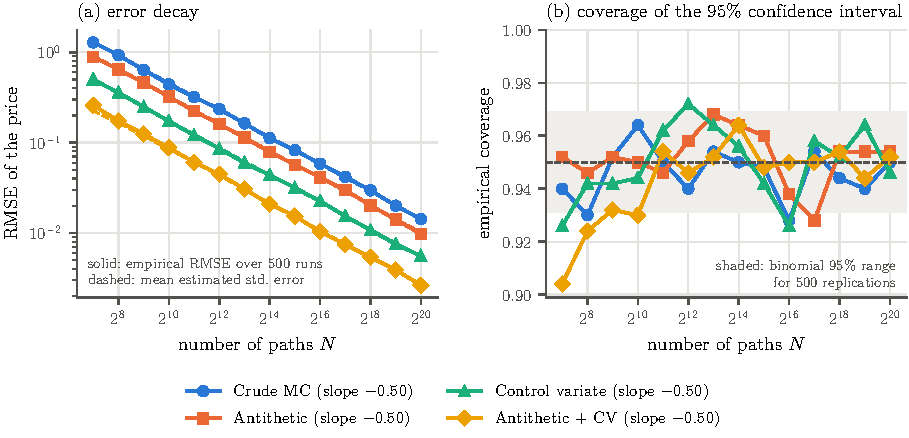
\includegraphics[width=\textwidth]{figures/convergence.pdf}
  \caption{(a) RMSE of the price over \Replications{} replications (markers) and average estimated standard
  error (dashed) against the number of paths; the slopes in the legend are fitted for $N \ge 2^{10}$.
  (b) Fraction of the replications whose 95\% confidence interval contains the Black--Scholes price.}
  \label{fig:convergence}
\end{figure}

\begin{figure}[ht]
  \centering
  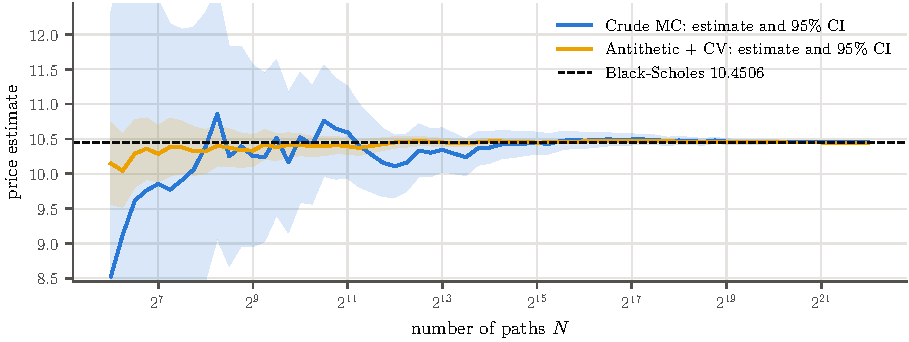
\includegraphics[width=\textwidth]{figures/running_estimate.pdf}
  \caption{One simulation of increasing size with its 95\% confidence band, crude estimator against the
  antithetic + control variate estimator. The runs are nested: the run of size $N$ is the prefix of all larger
  ones.}
  \label{fig:running}
\end{figure}

\subsection{Variance reduction}\label{sec:res-vr}

\Cref{tab:vr} compares the four estimators on the at-the-money call with $N = \TablePaths$ paths; timings are
the median of five interleaved runs. The control variate is strongly correlated with the payoff
($\hat\rho = \RhoCV$), and the measured VRF of \VRFCV{} coincides with the theoretical value
$1/(1-\hat\rho^2) = \TheoryVRFCV$ of \eqref{eq:cv}. The estimated coefficient $\hat\beta = \BetaCV$ is close to,
but not equal to, the Black--Scholes delta $\Phi(d_1) = 0.637$: it is the best \emph{linear} hedge of the payoff
at maturity, not the local sensitivity. Antithetic sampling halves the variance (VRF \VRFAnti) and, because it
draws half as many Gaussians, nearly quadruples the efficiency. The combination is by far the best: the
standard error falls from \CrudeSE{} to \BothSE{}, a variance reduction of \VRFBoth{} and an efficiency gain of
\EffBoth: a given accuracy is reached \EffBoth{} times faster.

\begin{table}[ht]
\centering
\caption{At-the-money call ($C = \BSPrice$), $N = \TablePaths$ payoff evaluations per method. $z$ is the error
in standard errors, $\hat\rho$ the correlation between payoff and control, VRF the variance reduction factor and
the efficiency gain is defined in \eqref{eq:efficiency}.}
\label{tab:vr}
\small
% Generated by scripts/make_figures.py -- do not edit by hand.
\begin{tabular}{lcrrrrr}
\toprule
Estimator & Price $\pm$ std.\ error & $z$ & $\hat\rho$ & VRF & Time (ms) & Efficiency \\
\midrule
Crude Monte Carlo & $10.4484 \pm 0.0072$ & $-0.30$ & -- & 1.00 & 34 & 1.00 \\
Antithetic variates & $10.4574 \pm 0.0051$ & $+1.35$ & -- & 2.00 & 18 & 3.69 \\
Control variate & $10.4539 \pm 0.0027$ & $+1.21$ & 0.925 & 6.89 & 37 & 6.30 \\
Antithetic + control variate & $10.4510 \pm 0.0013$ & $+0.33$ & 0.964 & 28.7 & 18 & 53.5 \\
\bottomrule
\end{tabular}

\end{table}

\Cref{fig:vr} shows how the gains depend on moneyness, for calls and puts. They are largest when the option is
deep in the money, where the payoff is nearly linear in $S_T$: the control variate then explains almost all of
the variance (VRF \VRFCVCallLow{} for the call struck at 70) and antithetic sampling is effective too
(\VRFAntiCallLow). Out of the money the payoff is zero on most paths, the correlation with any smooth
transformation of $Z$ collapses, and both methods bring little on their own (VRF \VRFAntiCallHigh{} and
\VRFCVCallHigh{} at $K = 130$). The put mirrors this picture. The combined estimator keeps a VRF above 10 for the
call over the whole range of strikes: once antithetic averaging has removed the odd part of the payoff, the
control variate still captures a large share of what remains. For production use, this suggests choosing a
control that matches the payoff, such as a vanilla option with a closed-form price, rather than the underlying
itself when pricing far out of the money.

\begin{figure}[ht]
  \centering
  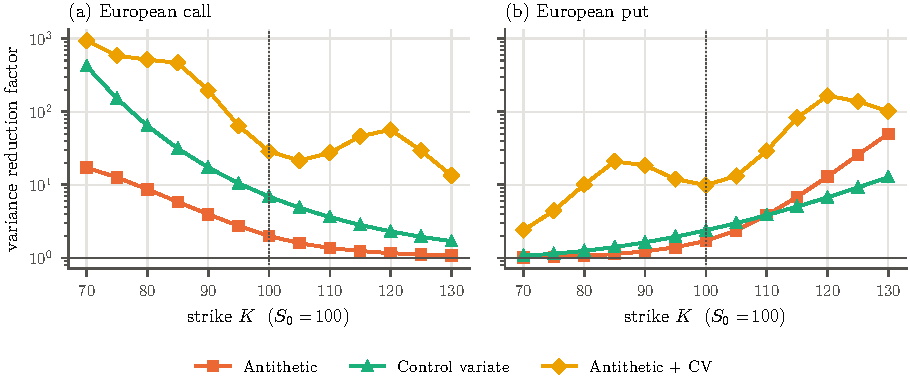
\includegraphics[width=\textwidth]{figures/variance_reduction.pdf}
  \caption{Variance reduction factor against strike for calls and puts ($N = \TablePaths$, logarithmic scale).
  The dotted line marks the money.}
  \label{fig:vr}
\end{figure}

\subsection{Greeks}\label{sec:res-greeks}

\Cref{tab:greeks} reports every estimator of the five Greeks with $N = \TablePaths$ paths and the default bumps
($h = 1\%$ of $S_0$ for Delta and Gamma, $10^{-3}$ for $\sigma$, one basis point for $r$, one day for $T$).
With common random numbers, every finite-difference estimate is within a few standard errors of the closed form.
With independent draws, the same bumps produce useless estimates: the variance is \DeltaCRNVarianceGain{} times
larger for Delta and \GammaCRNVarianceGain{} times larger for Gamma. For the first-order Greeks the CRN
estimates are practically identical to the pathwise ones, as expected from their path-by-path convergence, and
the likelihood-ratio estimator has a variance \DeltaLRVarianceRatio{} times larger for Delta.

\begin{table}[ht]
\centering
\caption{Monte Carlo Greeks of the at-the-money call, $N = \TablePaths$ paths; standard errors in parentheses.
FD: central finite difference with common random numbers (CRN) or independent draws.}
\label{tab:greeks}
\small
% Generated by scripts/make_figures.py -- do not edit by hand.
\begin{tabular}{lrrrrr}
\toprule
Greek & Closed form & FD, CRN & FD, independent & Pathwise & Likelihood ratio \\
\midrule
$\Delta$ (delta) & $0.636831$ & $0.63679$ & $0.6401$ & $0.63691$ & $0.63690$ \\
 &  & \footnotesize (0.00028) & \footnotesize (0.0051) & \footnotesize (0.00028) & \footnotesize (0.00072) \\[2pt]
$\Gamma$ (gamma) & $0.0187620$ & $0.018747$ & $0.038$ & n/a & $0.018761$ \\
 &  & \footnotesize (0.000052) & \footnotesize (0.018) &  & \footnotesize (0.000067) \\[2pt]
$\mathcal{V}$ (vega) & $37.5240$ & $37.537$ & $40.9$ & $37.536$ & $37.52$ \\
 &  & \footnotesize (0.037) & \footnotesize (5.1) & \footnotesize (0.037) & \footnotesize (0.13) \\[2pt]
$\rho$ (rho) & $53.2325$ & $53.237$ & $87$ & $53.238$ & $53.237$ \\
 &  & \footnotesize (0.023) & \footnotesize (51) & \footnotesize (0.023) & \footnotesize (0.065) \\[2pt]
$\Theta$ (theta) & $-6.41403$ & $-6.4155$ & $-7.7$ & $-6.4155$ & n/a \\
 &  & \footnotesize (0.0043) & \footnotesize (1.9) & \footnotesize (0.0043) &  \\
\bottomrule
\end{tabular}

\end{table}

The choice of the bump is studied in \cref{fig:greeks-bump}: for 21 relative bumps $h/S_0$ between $10^{-4}$
and $0.32$, the Delta and Gamma estimators are computed \GreekReplications{} times with $N = \GreekBumpPaths$
paths, and their RMSE against the closed form is plotted. The slopes predicted in \cref{sec:greeks} appear
clearly. With independent draws the error grows as $h^{-1}$ for Delta and $h^{-2}$ for Gamma when the bump
shrinks; the best attainable RMSE is \BestDeltaIndepRmse{} for Delta (at $h/S_0 \approx \BestDeltaIndepH$) and
\BestGammaIndepRmse{} for Gamma. With CRN the Delta error is flat for small bumps and equal to that of the
pathwise estimator (\DeltaPathwiseRmse), until the $\mathcal{O}(h^2)$ bias takes over beyond a few percent of
the spot. The CRN Gamma error decreases as $h^{-1/2}$, reaches its minimum \BestGammaRmse{} around
$h/S_0 \approx \BestGammaH$, then increases with the bias. At this optimal bump the CRN estimator beats the
likelihood-ratio Gamma (RMSE \GammaLikelihoodRatioRmse), which is unbiased but noisy. The practical lesson is
that, with common random numbers, finite differences are a robust default for first-order Greeks with a small
bump, whereas Gamma requires a bump of a few percent of the spot.

\begin{figure}[ht]
  \centering
  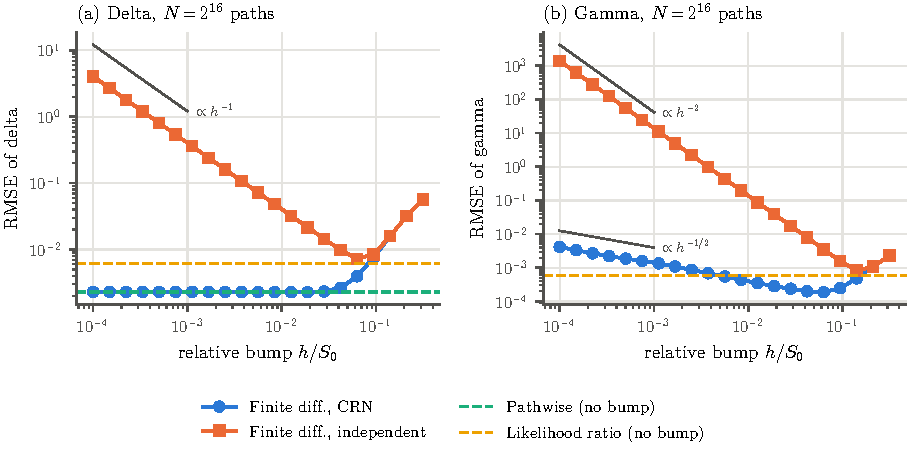
\includegraphics[width=\textwidth]{figures/greeks_bump.pdf}
  \caption{RMSE of the finite-difference Delta and Gamma against the relative bump, with common random numbers
  and with independent draws (\GreekReplications{} replications of $N = \GreekBumpPaths$ paths). Dashed
  horizontal lines: unbiased pathwise and likelihood-ratio estimators at the same budget. Grey segments: slopes
  predicted by the variance analysis of \cref{sec:greeks}.}
  \label{fig:greeks-bump}
\end{figure}

\subsection{Extension: arithmetic Asian option}\label{sec:res-asian}

The arithmetic Asian call pays $\big(\frac1n\sum_{k=1}^n S_{t_k} - K\big)^+$ on $n = 12$ monthly fixings and
has no closed form, which is the situation Monte Carlo is meant for. The path is simulated exactly on the fixing
grid. Its geometric counterpart, which pays on $G = (\prod_k S_{t_k})^{1/n}$, has a closed form because
$\ln G$ is Gaussian with mean $\ln S_0 + (r - q - \frac{\sigma^2}{2})T\frac{n+1}{2n}$ and variance
$\sigma^2 T\frac{(n+1)(2n+1)}{6n^2}$; it is an excellent control variate \citep{kemna1990}.
\Cref{tab:asian} confirms it: the correlation between the two payoffs exceeds 0.999 and the variance falls by a
factor of about \AsianVRFCV{} at the money, while the estimated coefficient $\hat\beta = \AsianBetaCV$ is close
to the value 1 used by Kemna and Vorst. Adding antithetic sampling brings no further variance reduction: at the
money the VRF even drops to \AsianVRFBoth, because the correlation of the pair averages (\AsianRhoBoth) is
slightly lower than that of single paths (\AsianRhoCV). It is nevertheless the most efficient estimator at
every strike, because it halves the number of Gaussian draws. The reference values are computed with
the combined estimator and $2^{25}$ paths.

\begin{table}[ht]
\centering
\caption{Arithmetic Asian call with 12 monthly fixings, $N = 2^{20}$ paths per estimator. The control variate
is the geometric Asian call with the same strike.}
\label{tab:asian}
\small
% Generated by scripts/make_figures.py -- do not edit by hand.
\begin{tabular}{llcrrr}
\toprule
Strike & Estimator & Price $\pm$ std.\ error & VRF & Efficiency & $\hat\rho$ \\
\midrule
90 & Crude Monte Carlo & $12.925 \pm 0.011$ & 1.00 & 1.00 & -- \\
 & Antithetic variates & $12.9219 \pm 0.0039$ & 7.46 & 11.4 & -- \\
 & Control variate & $12.91956 \pm 0.00026$ & 1\,727 & 1\,701 & 0.9997 \\
 & Antithetic + control variate & $12.91954 \pm 0.00029$ & 1\,398 & 2\,233 & 0.9973 \\
 & \textit{Reference value} & $12.919990 \pm 0.000051$ & & & \\
\midrule
100 & Crude Monte Carlo & $6.1619 \pm 0.0083$ & 1.00 & 1.00 & -- \\
 & Antithetic variates & $6.1599 \pm 0.0058$ & 2.08 & 3.28 & -- \\
 & Control variate & $6.15577 \pm 0.00023$ & 1\,301 & 1\,247 & 0.9996 \\
 & Antithetic + control variate & $6.15571 \pm 0.00024$ & 1\,197 & 1\,874 & 0.9991 \\
 & \textit{Reference value} & $6.156058 \pm 0.000043$ & & & \\
\midrule
110 & Crude Monte Carlo & $2.2937 \pm 0.0053$ & 1.00 & 1.00 & -- \\
 & Antithetic variates & $2.2926 \pm 0.0048$ & 1.22 & 1.86 & -- \\
 & Control variate & $2.29007 \pm 0.00021$ & 630 & 613 & 0.9992 \\
 & Antithetic + control variate & $2.29022 \pm 0.00021$ & 649 & 968 & 0.9991 \\
 & \textit{Reference value} & $2.290346 \pm 0.000037$ & & & \\
\bottomrule
\end{tabular}

\end{table}

\subsection{Extension: randomised quasi-Monte Carlo}\label{sec:res-qmc}

The $N^{-1/2}$ rate is a property of random sampling, not of the integration problem. Replacing the uniforms by
the van der Corput sequence in base 2, the first coordinate of the Sobol' sequence \citep{sobol1967}, and
applying a uniform random shift modulo 1 \citep{cranley1976} gives an unbiased estimator whose variance can be
measured over independent shifts \citep{lecuyer2002}. \Cref{fig:qmc} compares its RMSE over \Replications{}
shifts with the Monte Carlo estimators: the error now decays as $N^{\SlopeRQMC}$, and with $2^{20}$ points it is
\RQMCGainAtMax{} times smaller than that of crude Monte Carlo, a variance reduction of about
\RQMCVarianceGainAtMax. The rate is slightly below one, which is consistent with the integrand
$u \mapsto f\big(S_T(\Phi^{-1}(u))\big)$ being unbounded, hence of unbounded variation, near $u = 1$. In one
dimension this is a near-ideal case; for path-dependent payoffs in many dimensions the gain depends on the
effective dimension and calls for Sobol' points combined with a Brownian bridge construction
\citep[ch.~5]{glasserman2003}.

\begin{figure}[ht]
  \centering
  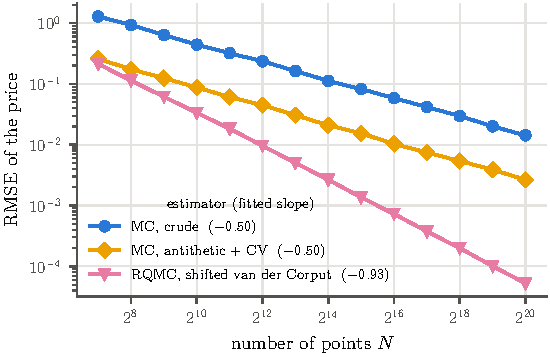
\includegraphics[width=0.62\textwidth]{figures/qmc.pdf}
  \caption{RMSE of the at-the-money call price: Monte Carlo estimators against randomly shifted van der Corput
  points (\Replications{} independent shifts per $N$). Fitted slopes in parentheses.}
  \label{fig:qmc}
\end{figure}

\subsection{Performance and reproducibility}

\Cref{tab:perf} reports the time needed to price the call with $\PerfPaths$ paths as a function of the number of
OpenMP threads (median of five runs). The kernel reaches \ThroughputSerial{} million paths per second on one
thread and \ThroughputParallel{} million with \ThreadsBest{} threads, a speed-up of \SpeedupMax. The scaling is
almost linear up to eight threads and slower beyond, because the processor combines four performance cores
(eight hardware threads) with eight slower efficiency cores. Dynamic scheduling of the blocks matters on such a
hybrid processor: with a static partition, the fast cores wait for the slow ones and 16 threads were measured
to be slower than 8. In every configuration the price is bitwise identical to the single-threaded one.

\begin{table}[ht]
\centering
\caption{Crude Monte Carlo price of the at-the-money call with $\PerfPaths$ paths against the number of threads.}
\label{tab:perf}
% Generated by scripts/make_figures.py -- do not edit by hand.
\begin{tabular}{rrrrc}
\toprule
Threads & Time (ms) & Paths per second & Speed-up & Bitwise identical \\
\midrule
1 & 1809 & $9.3\times 10^6$ & 1.00 & yes \\
2 & 903 & $18.6\times 10^6$ & 2.00 & yes \\
4 & 456 & $36.8\times 10^6$ & 3.97 & yes \\
8 & 251 & $66.8\times 10^6$ & 7.20 & yes \\
12 & 172 & $97.4\times 10^6$ & 10.50 & yes \\
16 & 134 & $124.9\times 10^6$ & 13.47 & yes \\
\bottomrule
\end{tabular}

\end{table}

% =====================================================================================================
\section{Conclusion}

Measured against the Black--Scholes closed form, the Monte Carlo estimators behave as the theory predicts: the
error decays as $N^{-1/2}$ with slopes within $0.01$ of $-1/2$, the estimated standard errors match the true
RMSE within a few percent, and the confidence intervals reach their nominal coverage once $N$ exceeds a few
thousand paths. Variance reduction changes the constant, not the rate, and must be judged on efficiency rather
than variance alone: combining antithetic variates with a control variate on the terminal price divides the
cost of a given accuracy by \EffBoth{} at the money, and a well-chosen control (the geometric Asian option) by
more than a thousand for an arithmetic Asian. For Greeks, common random numbers are not an optimisation but a
requirement, and the bump size must be chosen according to the smoothness of the payoff.

Natural extensions of this code base are models without exact simulation, such as Heston's stochastic
volatility \citep{heston1993}, where the discretisation bias has to be balanced against the statistical error;
American options with the Longstaff--Schwartz regression \citep{longstaff2001}; multidimensional Sobol' points
with a Brownian bridge; and adjoint algorithmic differentiation, which delivers all pathwise Greeks at a small
multiple of the cost of the price \citep{giles2006}.

\appendix
\section{Reproducing the results}\label{app:reproduce}

Every number, table and figure of this report is generated from the repository \repo:
\begin{verbatim}
cmake -S . -B build -DCMAKE_BUILD_TYPE=Release
cmake --build build --config Release
ctest --test-dir build -C Release        # unit tests
build/run_experiments results            # ~5 min on 16 threads
python scripts/make_figures.py           # figures, tables, macros
latexmk -pdf -cd report/report.tex
\end{verbatim}
The experiments are deterministic: rerunning them reproduces the statistical results exactly; only the
timings depend on the machine.

\bibliographystyle{plainnat}
\bibliography{references}

\end{document}
